%\begin{figure}[t]
%	\centering
%	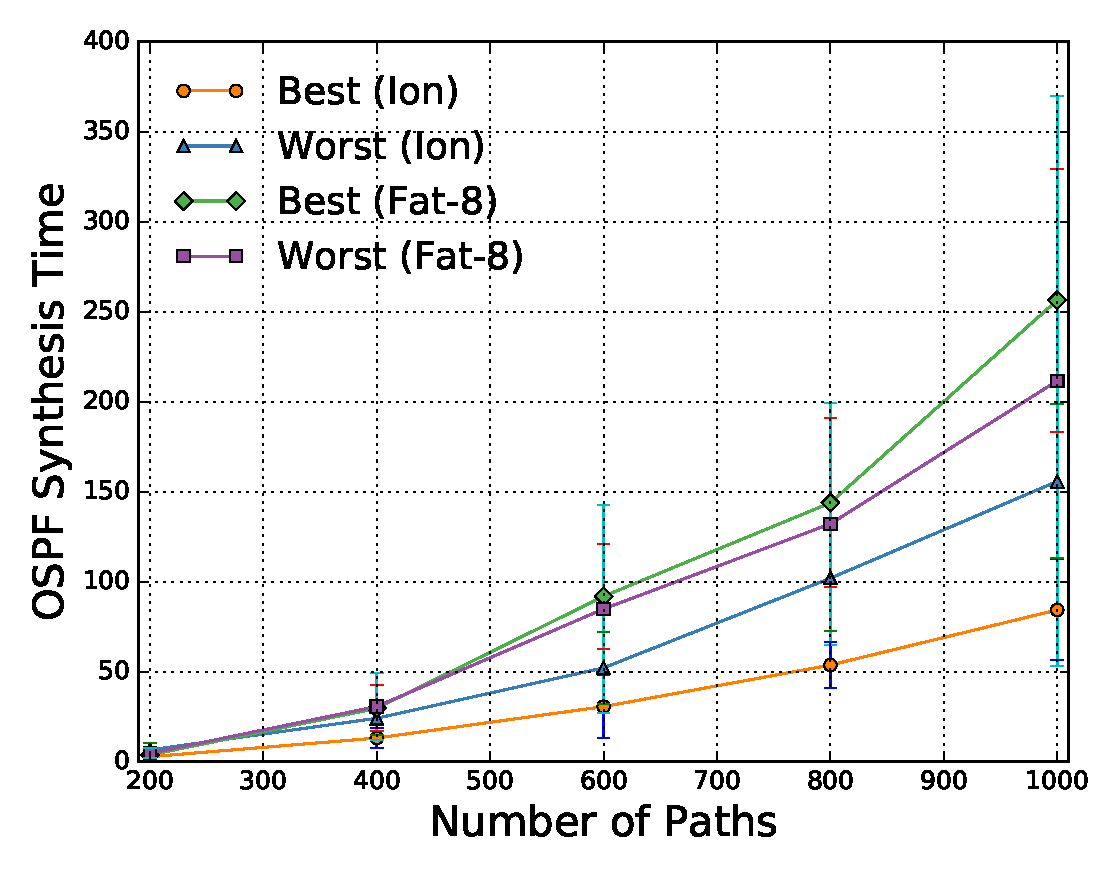
\includegraphics[width=0.7\columnwidth]{figures/ospfSynthesisTimeMCMC.eps}
%	\compactcaption{MCMC OSPF Synthesis time}
%	\label{fig:ospfmcmc}
%\end{figure}
\begin{figure*}
	\centering
	\subfloat[Synthesis Time]
	{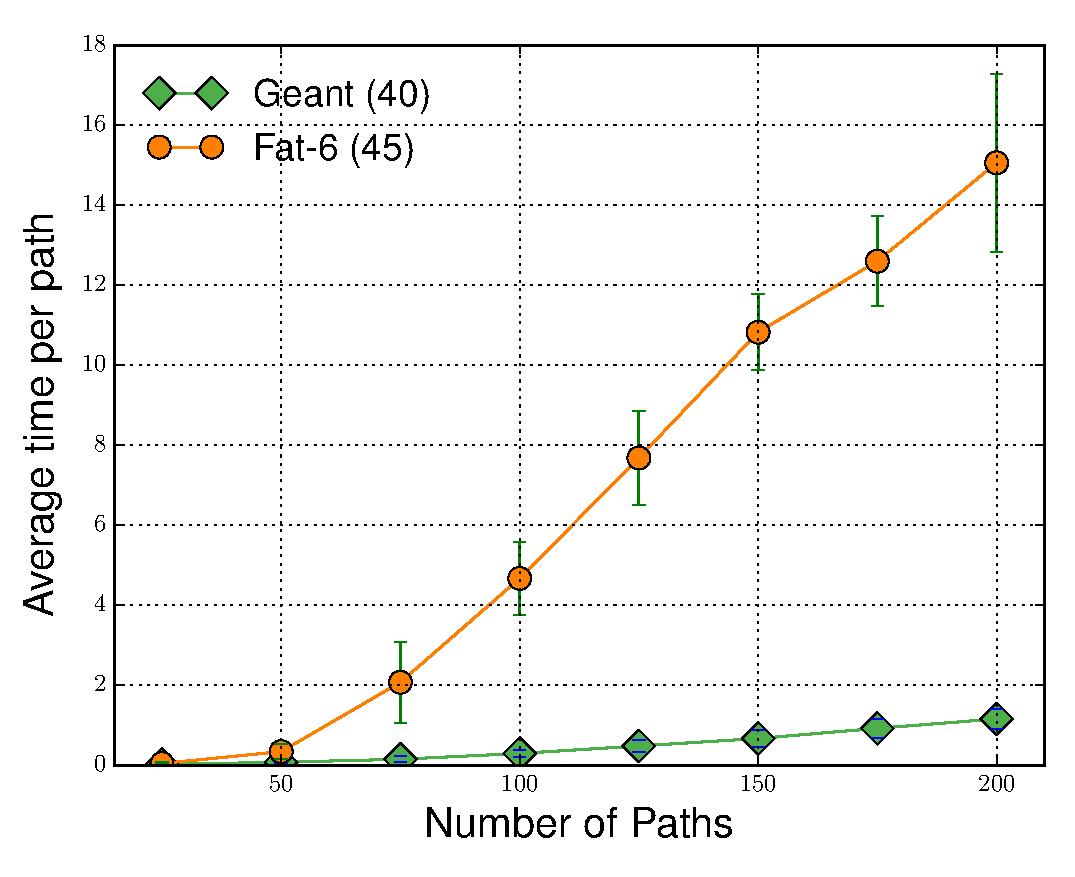
\includegraphics[width=0.66\columnwidth]{figures/ospfTime.eps}}
	\subfloat[Number of Route Filters]
	{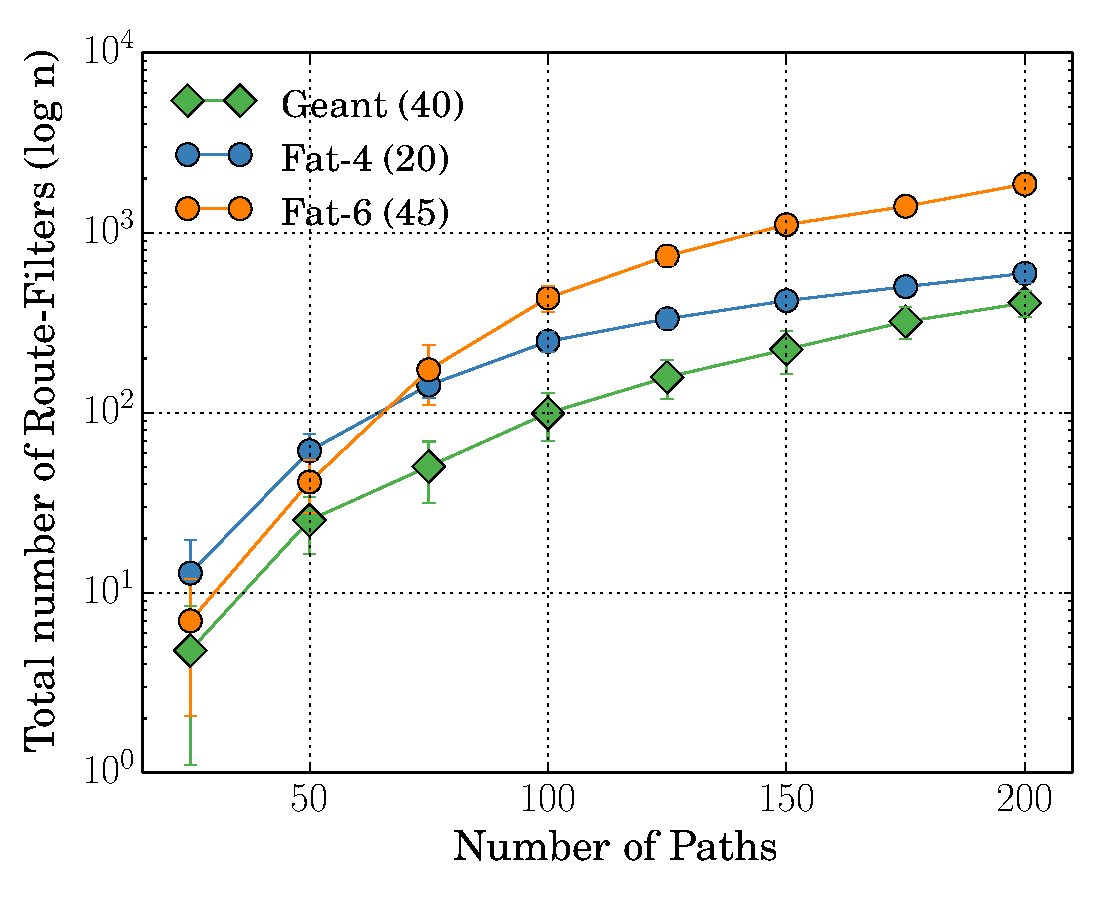
\includegraphics[width=0.66\columnwidth]{figures/ospfRF.eps}}
	\subfloat[Endpoint Resilience]
	{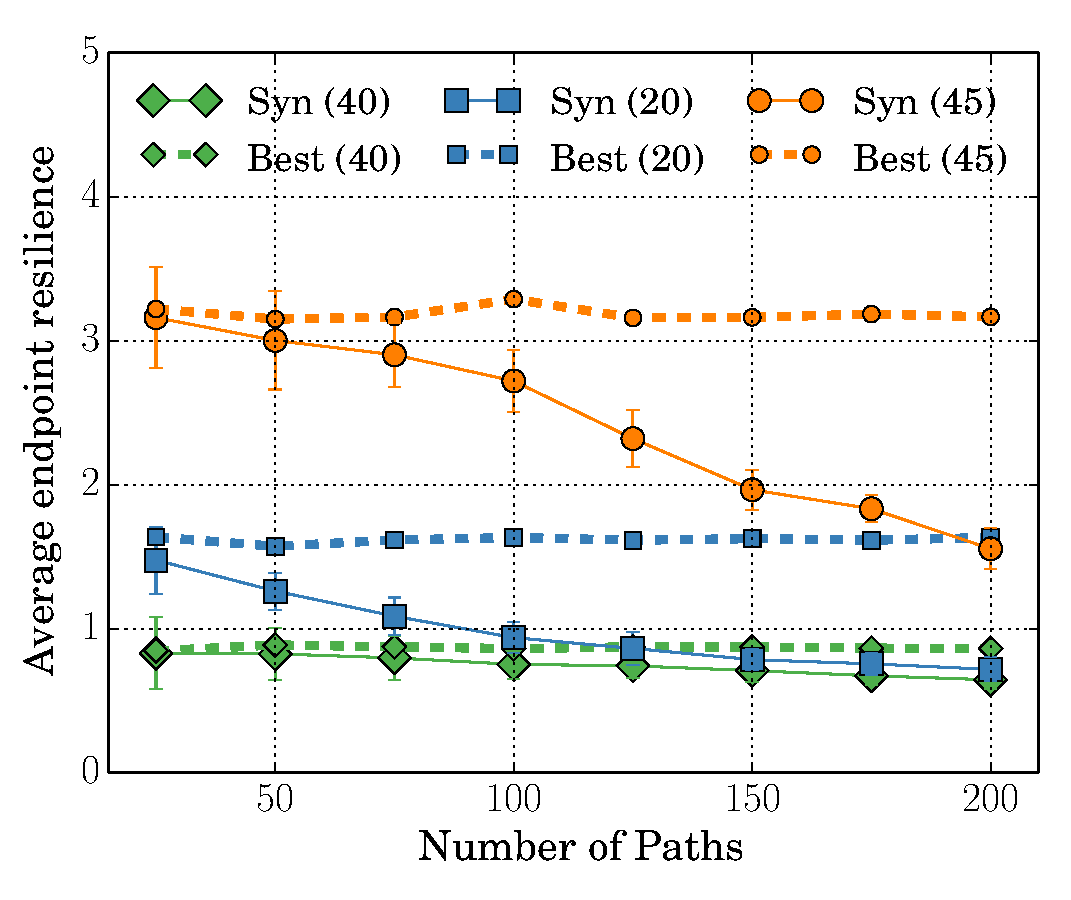
\includegraphics[width=0.66\columnwidth]{figures/ospfAvgRes.eps}}
	\compactcaption{\label{fig:ospfeval}
		OSPF Synthesis evaluation}
\end{figure*}


\begin{figure}
	\centering
	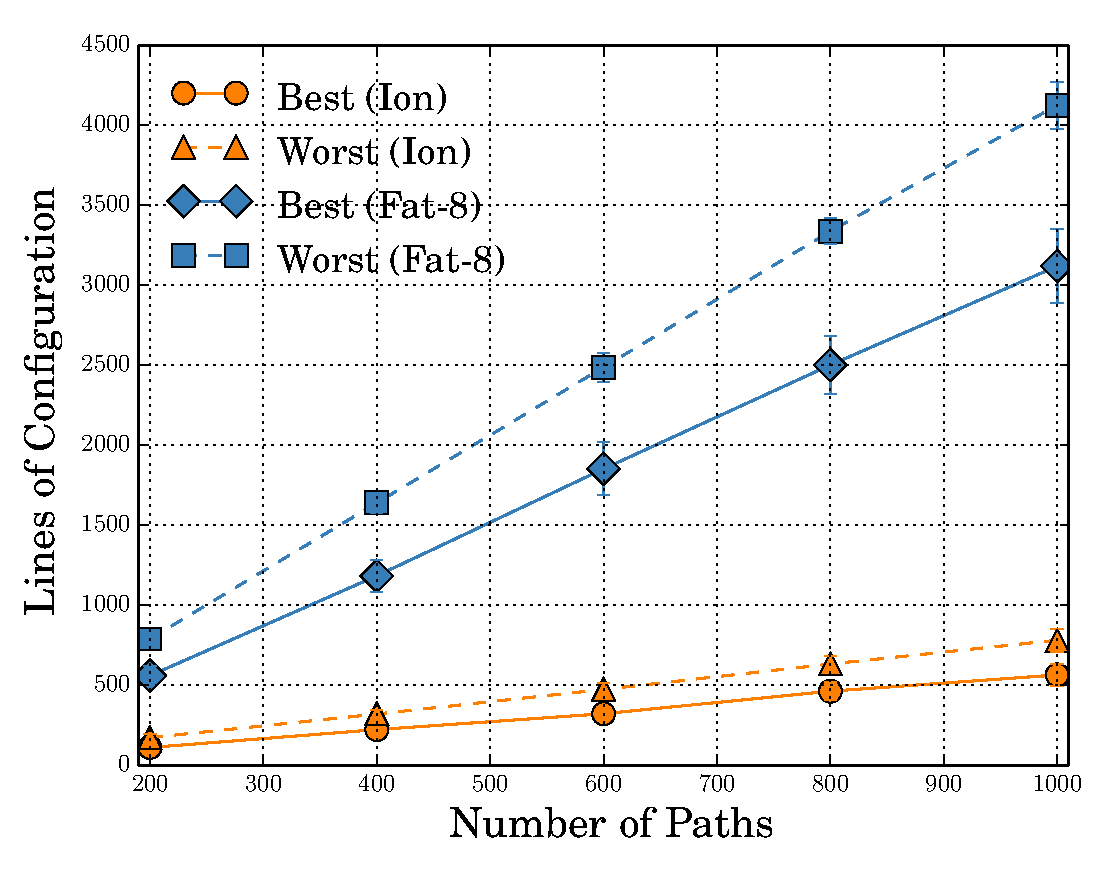
\includegraphics[width=0.7\columnwidth]{figures/confMCMC.eps}
	\compactcaption{MCMC Lines of Conf}
	\label{fig:confmcmc}
\end{figure}

\begin{figure}
	\centering
	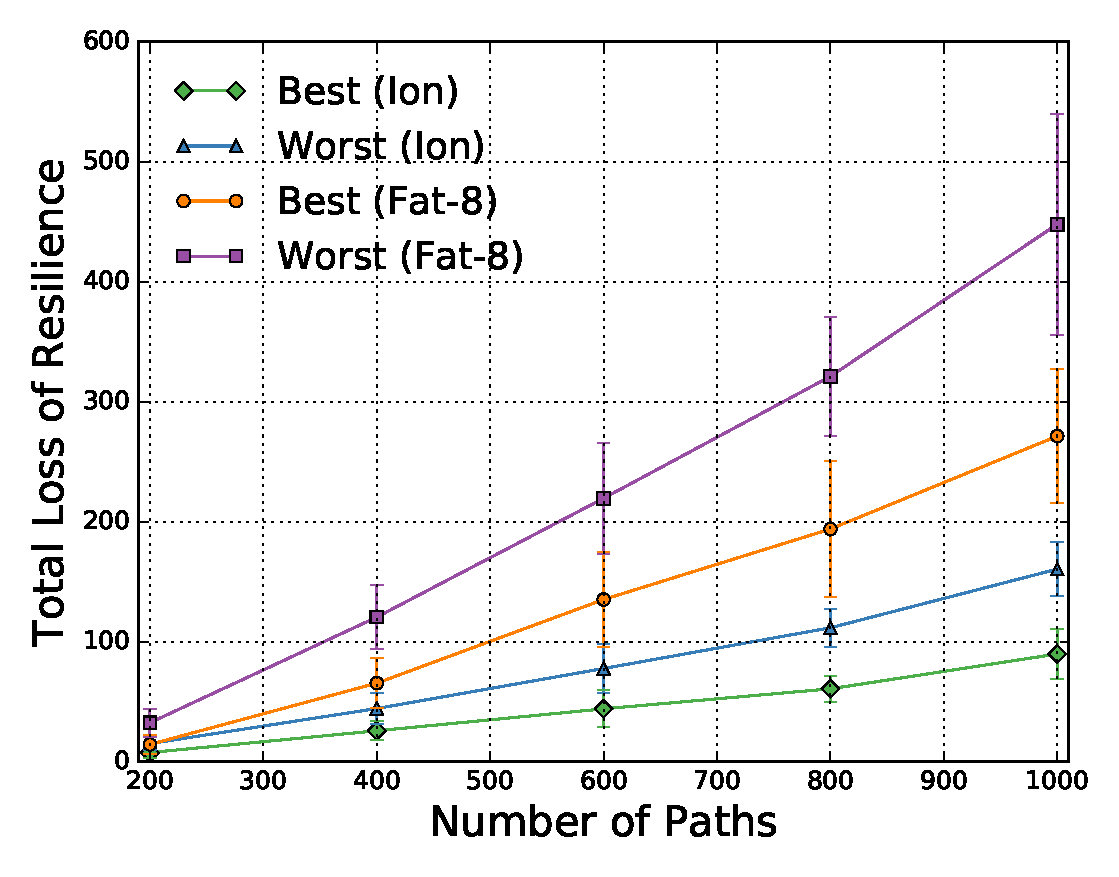
\includegraphics[width=0.7\columnwidth]{figures/TRLMCMC.eps}
	\compactcaption{MCMC TRL}
	\label{fig:trlmcmc}
\end{figure}

\begin{figure}
	\centering
	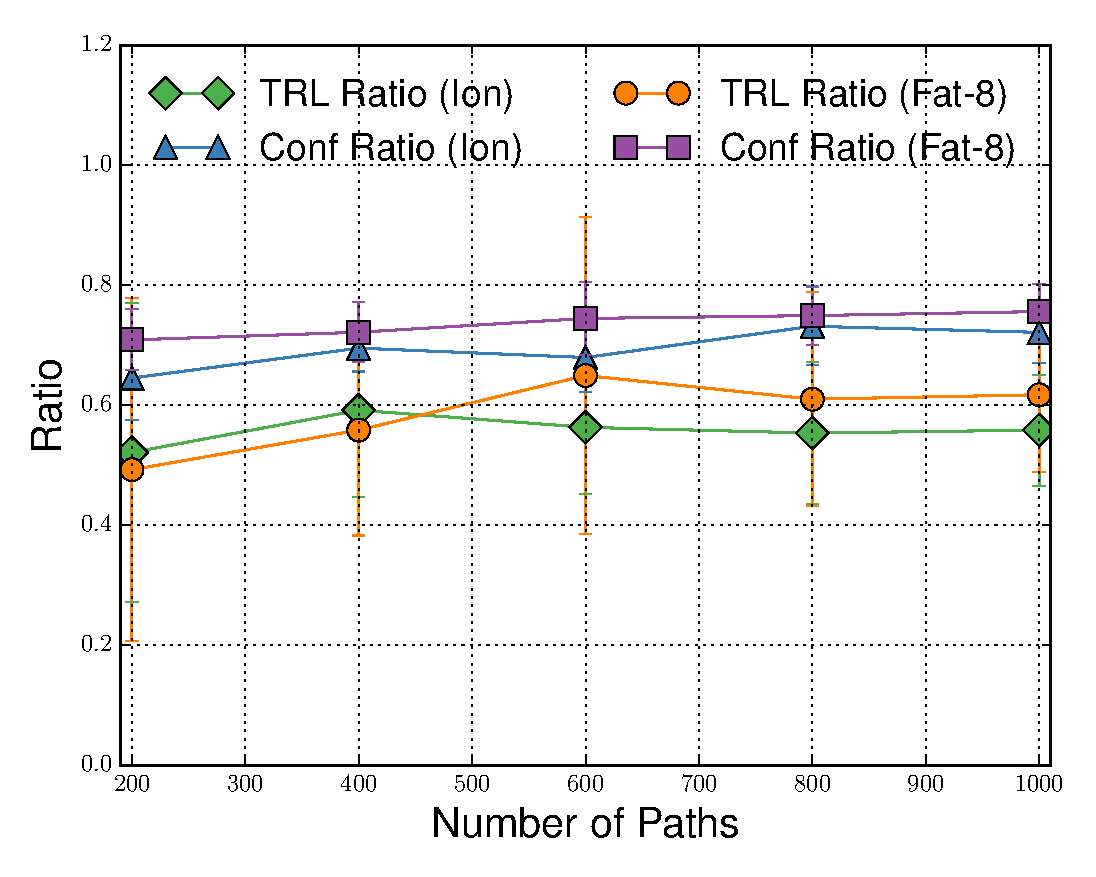
\includegraphics[width=0.7\columnwidth]{figures/ratioMCMC.eps}
	\compactcaption{MCMC Ratios}
	\label{fig:ratiomcmc}
\end{figure}




\section{Evaluation}
 \label{sec:evaluation}
 
 We implemented a full working
 prototype of \name in Python, which works as a standalone
 system or can be integrated with \genesis. For a given
 workload, \name outputs abstract configurations, which
 specifies the assignment of domains to different routers,
 the static routes, BGP configuration variables (local 
 preferences and iBGP filters), and the OSPF link weights
 and route-filters for each domain, which can be 
 translated to actual device configurations using templates~\cite{template}.
 \name uses the Gurobi LP solver~\cite{gurobi} for synthesis of 
 OSPF weights and filters. 
 
In this section, we evaluate \Name using
%\loris{really don't like the word realistic}
enterprise-scale data
center fat-tree topologies~\cite{fattree} of different 
sizes, and ISP topologies from the Internet Topology Zoo 
dataset~\cite{zoo} and ISP topologies.  
Specifically, we ask:
\begin{itemize}
	\item What is the performance of \Name's OSPF synthesis
	algorithm? How does synthesis time and resilience properties 
	vary with size and type of the network and number of paths? (\secref{sec:ospfeval})
	
	\item How well does \name's stochastic domain assignment 
	search work in optimizing configuration overhead
	and maximizing endpoint resilience of the paths? (\secref{sec:mcmceval})
	
	\item How does \name perform in an end-to-end scenario, going
	from policies to configurations in conjuction with \genesis? 
	(\secref{sec:genzep})
\end{itemize}
All experiments were conducted using a
32-core Intel-Xeon 2.40GHz CPU machine and
128GB of RAM.

\subsection{OSPF Synthesis Performance}
To benchmark our performance of \name's OSPF synthesis,
we consider three topologies: Geant ISP topology with 40 routers,
and 2 fat-tree topologies with 20 (Fat-4) and 45 routers (Fat-6). 
These sizes are consistent with operator preferences to restrict
the size of a domain to under 50 routers (OSPF does not scale w
well as domain size increases). We generate $n$ random input paths for
$n/4$ destinations spread across the topology and 
lengths in range [3,5]. For each metric, we perform 20 experiments
and report average and standard deviation. 

\noindent\textbf{Synthesis Time.}~~~\Cref{fig:ospfeval}(a) 
shows the synthesis time for increasing number of paths. 
The time taken for Fat-6 is much greater than Fat-4 or Geant
due to more number of links, therefore there are more link weights
to synthesize, and greater alternate paths to add constraints for. 
For Geant, we can sybthesize weights and filters in 200 seconds 
for 200 paths, thus OSPF synthesis is effective for ISP topologies
which have lesser links than datacenter topologies. 
\Cref{fig:ospfeval}(b) shows the number of filters synthesized. 
As the time taken is dependent on the number of iterations of
the route-filter learning procedure, the number of filters
shows a similar trend to OSPF synthesis time. On average, 2 route-filters
are required for each path in the Geant topology. 

\noindent\textbf{Endpoint Resilience.}~~~While the number of 
filters is related to synthesis time, our OSPF synthesis picks
filters which have the least effect on endpoint resilience, as it  
is a more important metric than the number of filters. We express this
by computing the average of $t-resilience$ for each endpoint considering
the filters ($t-resilience$ = $t+1$ edge-disjoint backup paths between the 
endpoints).
\Cref{fig:ospfeval}(c) shows the average
endpoint resilience obtained by \name (solid traces) 
compared to the best endpoint resilience (achieved
if there were no filters). For Geant, the endpoint 
resilience obtained by \name trails the best by a small margin,
even though 2 route-filters were required for each path. For
Fat-4 and Fat-6, there is a significant difference between \name's 
and the best resilience, however, we are able to achieve greater than
50 percent of the resilience offered by the topology. 